\section{Introduction}

Obfuscation represents a realistic and challenging deployment condition for code models, appearing frequently in malware triage, minified production code, and clone detection systems. Fine-tuning models on obfuscated output prediction yields an easy initial result: a massive +18.09 point improvement on the seen ladder. If that were the end of the story, this paper would simply be an engineering note.

However, real-world obfuscators do not rely on isolated transformations; they stack them. This raises the critical question of whether single-transform competence actually composes. We operationalize this question by testing three composition methods. The result is a sharp dissociation rather than a simple failure: while routing adds nothing and merging reduces performance, broad data coverage successfully generalises to seen stacked inputs (+3.49 points) but severely taxes performance on unseen transform families ($-3.79$ points).

To explain this phenomenon, we demonstrate that adaptation anchors strictly on the surface a transform leaves behind, rather than on the semantics it preserves. This is most evident when evaluating two independent mechanisms of a single obfuscation family that fail to transfer to each other, and when the entire performance gain collapses when the exact same programs are evaluated backwards. Consequently, we propose a remedy: if the failure stems from surface anchoring, we must anchor the model to clean-code behaviour instead. We introduce a paired-consistency objective that successfully removes the unseen-family costs without claiming spurious new capability, ultimately providing a Pareto improvement for robust code interpretation.

\begin{figure}
    \centering
    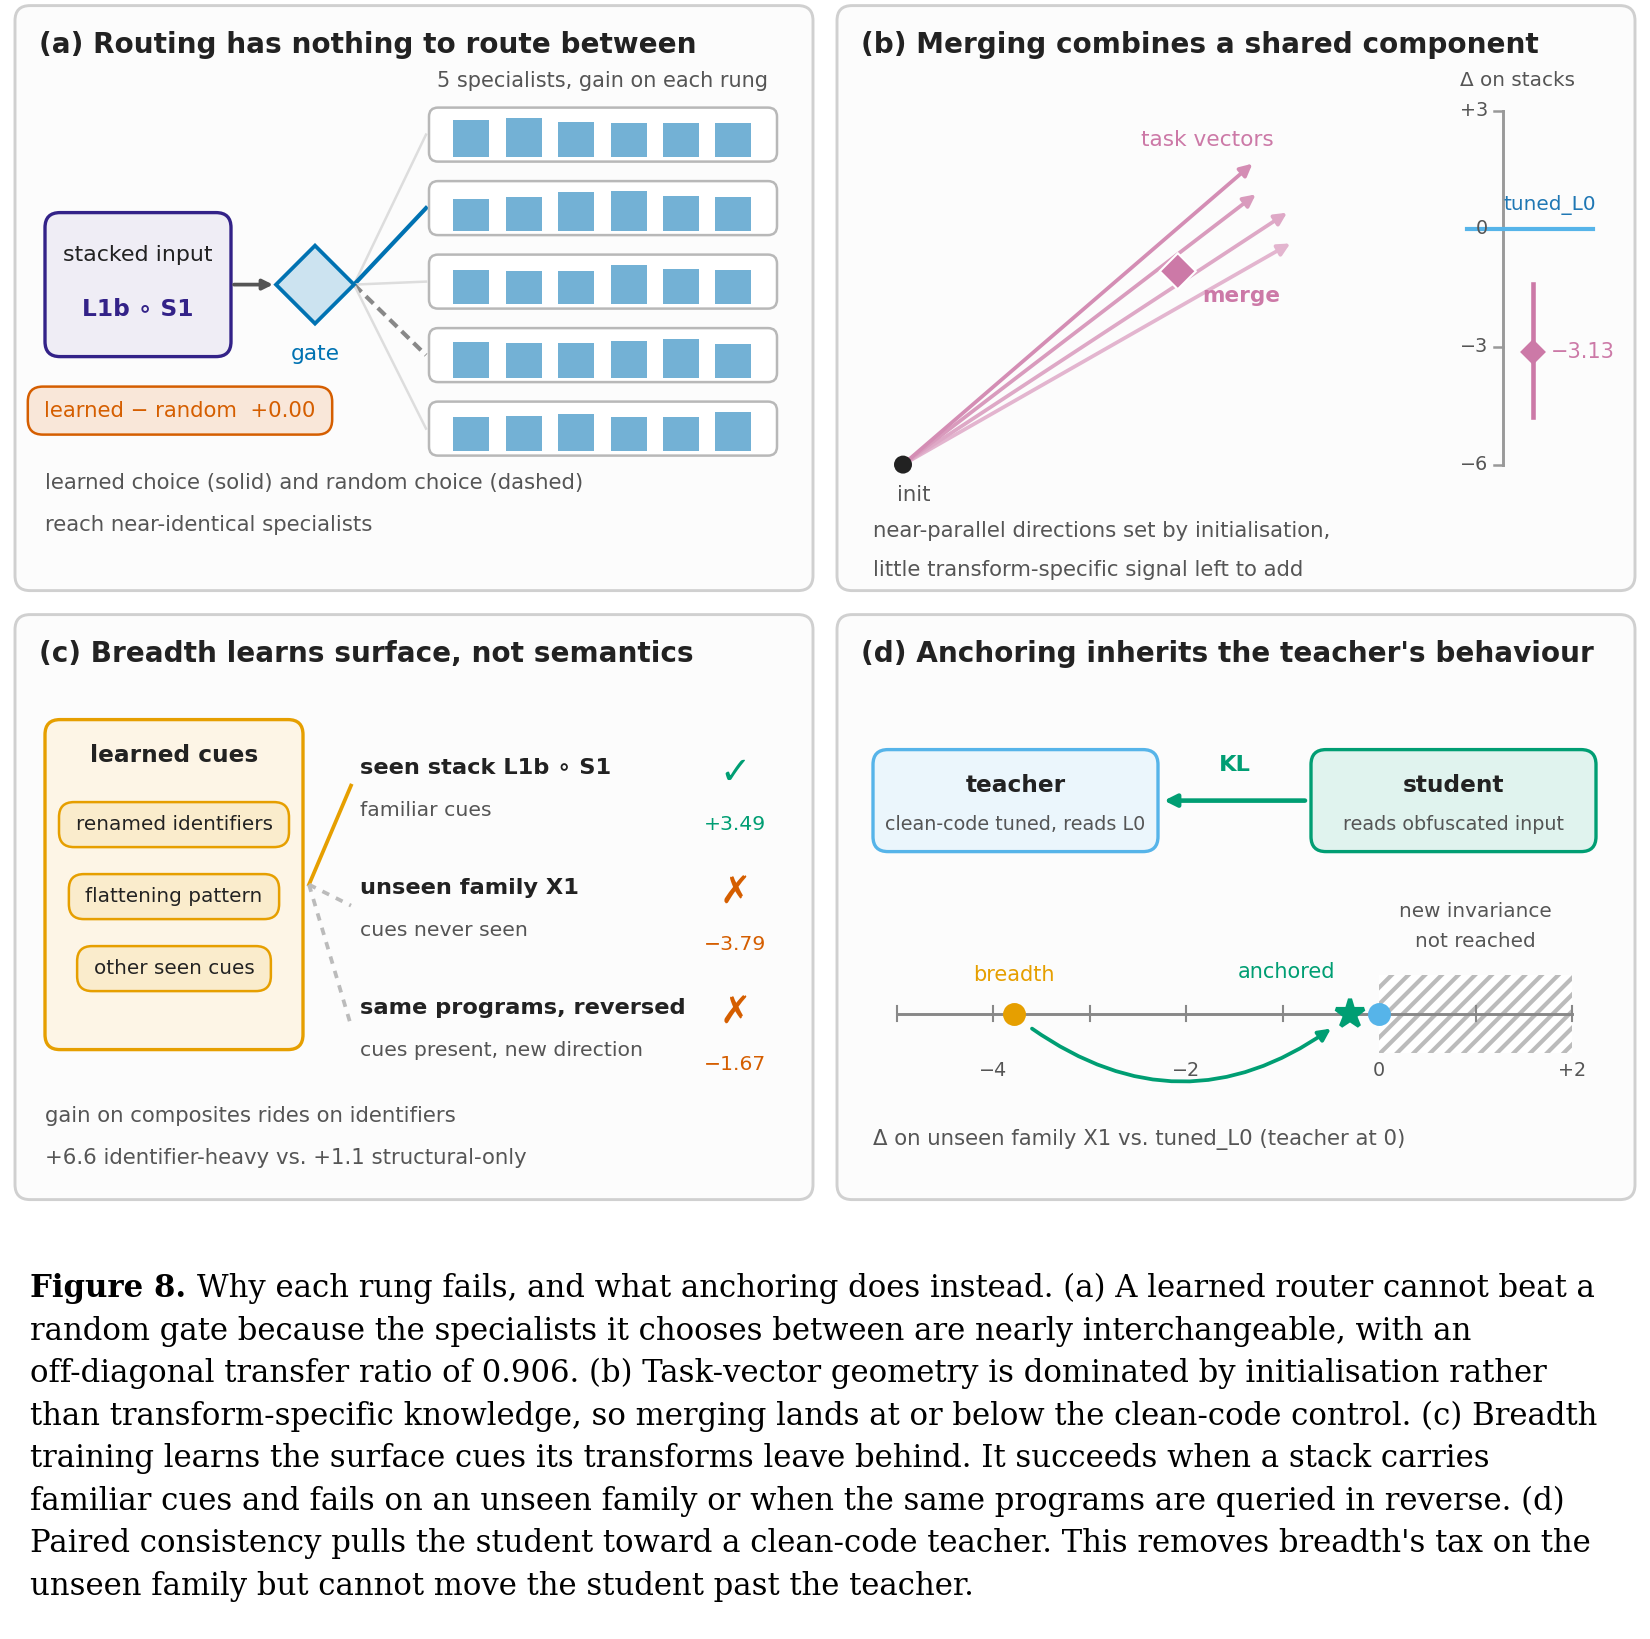
\includegraphics[width=1\linewidth]{figures/fig08_why_methods_fail.png}
    \caption{Enter Caption}
    \label{fig:placeholder}
\end{figure}

We analyze the following Research Questions: 
\begin{itemize}
   \item \textbf{RQ1: Do simple composition strategies work?} We evaluate baseline approaches building upon single compositions---including prompting combinations, inference-time routing, and weight-space merging. We show that these simple approaches that attempt to recombine single-transform competence fundamentally fail or suffer severe unseen-family taxes because they over-fit to superficial surface cues rather than underlying semantics.
    \item \textbf{RQ2: Can we achieve composition through a specialized loss term?} We introduce a paired-consistency objective designed to remove the generalization costs by forcing the model's representations to align with a clean-code-tuned teacher, anchoring it away from superficial cues.
    \item \textbf{RQ3: Which approaches achieve true robustness?} We subject the resulting anchored model to rigorous stress tests (deeper stacks, second languages, reverse tasks, and unseen families) to establish strict bounds on our claims, determining whether the objective creates genuine algorithmic invariance.
\end{itemize}

\red{add baseline by showing that the baseline doesn't work. 
Changing the Prompt, ICL 
run the baseline on the clean code 
}